% --------------------------------------------------------------
%     DENNE MALEN ER LAGET AV MARTIN SORIA RØVANG
%     TIL BRUK FOR OPPGAVELØSNINGER OG RAPPPRTER
%     GITHUB: github.com/martinrovang
% --------------------------------------------------------------


\documentclass[10pt]{article}
\usepackage{amsmath,amsthm,amssymb}
\usepackage{float}
\usepackage[norsk]{babel}
\usepackage[table]{xcolor}
\usepackage{color}
\usepackage{graphicx}
\usepackage{listings}
\usepackage{natbib}
\usepackage[utf8]{inputenc}
\usepackage{imakeidx}
\usepackage[a4paper]{geometry}
\usepackage[myheadings]{fullpage}
\usepackage{fancyhdr}
\usepackage{lastpage}
\usepackage{graphicx, wrapfig, subcaption, setspace, booktabs}
\usepackage[T1]{fontenc}
\usepackage[font=small, labelfont=bf]{caption}
\usepackage{fourier}
\usepackage[protrusion=true, expansion=true]{microtype}
\usepackage{url, lipsum}
\usepackage{tgbonum}
\usepackage{hyperref}
\usepackage{xcolor}
\usepackage[most]{tcolorbox}
\usepackage{mathtools}
\usepackage[page]{totalcount}
\usepackage{lastpage}


\newcommand{\HRule}[1]{\rule{\linewidth}{#1}}
\onehalfspacing
\setcounter{tocdepth}{5}
\setcounter{secnumdepth}{5}
\newcommand{\vect}[1]{\boldsymbol{#1}}

\definecolor{codegreen}{rgb}{0,0.6,0}
\definecolor{codegray}{rgb}{0.5,0.5,0.5}
\definecolor{codepurple}{rgb}{0.58,0,0.82}
\definecolor{backcolour}{rgb}{0.95,0.95,0.92}
\definecolor{skyblue}{rgb}{0.950, 1, 1}

\lstdefinestyle{mystyle}{
    backgroundcolor=\color{backcolour},   
    commentstyle=\color{codegreen},
    keywordstyle=\color{magenta},
    numberstyle=\tiny\color{codegray},
    stringstyle=\color{codepurple},
    basicstyle=\footnotesize,
    breakatwhitespace=false,         
    breaklines=true,                 
    captionpos=b,                    
    keepspaces=true,                 
    numbers=left,                    
    numbersep=5pt,                  
    showspaces=false,                
    showstringspaces=false,
    showtabs=false,                  
    tabsize=2,
    frame=single,
    %keywordstyle=\color{blue},
    language=Python,
    backgroundcolor = \color{skyblue}
}
 
\lstset{style=mystyle}
\lstset{
    basicstyle=\footnotesize\ttfamily,
  identifierstyle=\bfseries\color{green!40!black},
  commentstyle=\itshape\color{purple!40!black},
  keywordstyle=\color{blue},
  stringstyle=\color{orange},
}

\newcommand{\N}{\mathbb{N}}
\newcommand{\Z}{\mathbb{Z}}
 
\newenvironment{theorem}[2][Theorem]{\begin{trivlist}
\item[\hskip \labelsep {\bfseries #1}\hskip \labelsep {\bfseries #2.}]}{\end{trivlist}}
\newenvironment{lemma}[2][Lemma]{\begin{trivlist}
\item[\hskip \labelsep {\bfseries #1}\hskip \labelsep {\bfseries #2.}]}{\end{trivlist}}
\newenvironment{exercise}[2][Exercise]{\begin{trivlist}
\item[\hskip \labelsep {\bfseries #1}\hskip \labelsep {\bfseries #2.}]}{\end{trivlist}}
\newenvironment{problem}[2][Problem]{\begin{trivlist}
\item[\hskip \labelsep {\bfseries #1}\hskip \labelsep {\bfseries #2.}]}{\end{trivlist}}
\newenvironment{question}[2][Question]{\begin{trivlist}
\item[\hskip \labelsep {\bfseries #1}\hskip \labelsep {\bfseries #2.}]}{\end{trivlist}}
\newenvironment{corollary}[2][Corollary]{\begin{trivlist}
\item[\hskip \labelsep {\bfseries #1}\hskip \labelsep {\bfseries #2.}]}{\end{trivlist}}

\newenvironment{solution}{\begin{proof}[Solution]}{\end{proof}}
    
\makeindex[columns=3, title=Alphabetical Index, intoc]


% --------------------------------------------------------------
%                         Headers and footers
% --------------------------------------------------------------
\fancyhf{}
\pagestyle{fancy}
\rhead{Martin Soria Røvang}
\lhead{STA-2003-Tidsrekker}
\rfoot{Side \thepage \, av \pageref{LastPage}}
\renewcommand{\headrulewidth}{0.3pt}
\usepackage{amssymb}
\usepackage{gensymb}
\usepackage{amsmath}
\usepackage[section]{placeins}

\begin{document}
% --------------------------------------------------------------
%                         FRONTPAGE
% --------------------------------------------------------------
{\fontfamily{cmr}\selectfont
\title{ \normalsize \textsc{}
		\\ [1.0cm] % How much upper margin
		%\HRule{0.5pt} \\
        \LARGE \textbf{\uppercase{Obligatorisk Oppgave 2}
        \HRule{0.5pt} \\ [0.5cm]
        STA-2003-Tidsrekker
        %\HRule{2pt} \\ [0.5cm]
        \\
		\normalsize \today \vspace*{5\baselineskip}}
		}

        \date{}
\author{
		Martin Soria R�vang \\ 
        Universitetet i Troms�\\}

% \begin{titlepage}
\clearpage\maketitle
\vspace{0.2\textheight}
{\centering
Inneholder \pageref{LastPage} \, sider, inkludert forside.\par
}
\thispagestyle{empty}
% \end{titlepage}

\newpage
\tableofcontents
% --------------------------------------------------------------
%                         Start here
% --------------------------------------------------------------

% \cite{alpaydin_2014}
\newpage

\section{Oppgave}
\subsection{a}

Har prosessen,
\begin{equation}
    x(t) = x_{1}(t) + x_{2}(t)
    \label{starteq}
\end{equation}

,disse er \emph{ukorrelerte} og \emph{stasjon\ae re} prosesser med forventning $E[x_{1}] = E[x_{2}] = 0$. 

Vi har Wiener-Khinchin theoremene,

\begin{equation}
    S_{xx}(f) = \mathcal{F}\{R_{xx}(\tau)\} = \int_{\infty}^{\infty}R_{xx}(\tau)e^{-i2\pi f\tau}\,d\tau
\end{equation}
\begin{equation}
    R_{xx}(\tau) = \mathcal{F}^{-1}\{S_{xx}(f)\} = \int_{\infty}^{\infty}S_{xx}(f)e^{i2\pi f\tau}\,df
\end{equation}

Her er $\mathcal{F}$ Fourier transormasjon. Bruker at,

\begin{equation}
    R_{xx}(\tau) = E[x_{t+\tau }x_{t}]
\end{equation}

L\o ser vi denne med tanke p� ligning (\ref{starteq}) f�r vi,

\begin{equation}
    R_{xx}(\tau) = E[(x_{1}(t+h) + x_{2}(t+h)  )(x_{1}(t) + x_{2}(t)) ]
\end{equation}

Som gir,

\begin{equation}
    R_{xx}(\tau) = E[x_{1}(t+h)x_{1}(t)] + E[x_{1}(t+h)x_{2}(t+h)] + E[x_{1}(t+h)x_{2}(t)] + E[x_{2}(t+h)x_{2}(t)]
\end{equation}

Siden prosessene er ukorrelerte vil man kunne separere forventingene, $E[x_{1}(t+h)]E[x_{2}(t+h)]$

Dette gir da,

\begin{equation}
    R_{xx}(\tau) = E[x_{1}(t+h)x_{1}(t)] + E[x_{1}(t+h)]E[x_{2}(t+h)] + E[x_{1}(t+h)]E[x_{2}(t)] + E[x_{2}(t+h)x_{2}(t)]
\end{equation}

Dette kan separeres slik at,

\begin{equation}
    R_{xx}(\tau) = E[x_{1}(t+h)x_{1}(t)] + E[x_{1}(t+h)]E[x_{2}(t+h)] + E[x_{1}(t+h)]E[x_{2}(t)] + E[x_{2}(t+h)x_{2}(t)]
\end{equation}


Siden $R_{x_{1}x_{1}}(\tau) = E[x_{1}(t + \tau)x_{1}(t)]$ f�r vi,

\begin{equation}
    R_{xx}(\tau) = R_{x_{1}x_{1}}(\tau) + E[x_{1}(t+h)]E[x_{2}(t+h)] + E[x_{1}(t+h)]E[x_{2}(t)] + R_{x_{2}x_{2}}(\tau)
\end{equation}

Vet at forventningen til prosessene er null, $E[x_{1}(t+h)]E[x_{2}(t+h)] = 0$ og $ E[x_{1}(t+h)]E[x_{2}(t)]$,

\begin{equation}
    R_{xx}(\tau) = R_{x_{1}x_{1}}(\tau) + R_{x_{2}x_{2}}(\tau)
\end{equation}

Siden vi har summer kan vi dele integralet opp i sum,


\begin{equation}
    S_{xx}(f) = \underbrace{\int_{\infty}^{\infty}R_{x_{1}x_{1}}(\tau)e^{-i2\pi f\tau}\,d\tau}_{= S_{x_{1}x_{1}}(f)} + \underbrace{\int_{\infty}^{\infty}R_{x_{2}x_{2}}(\tau)e^{-i2\pi f\tau}\,d\tau}_{= S_{x_{2}x_{2}}(f)}
\end{equation}


\subsection{b}

I figur(\ref{taskb}) ser vi tidsrekken i �verste vindu, periodogram, og periodogram med hann vindu.

\begin{figure}[hbt!]
{\centering
    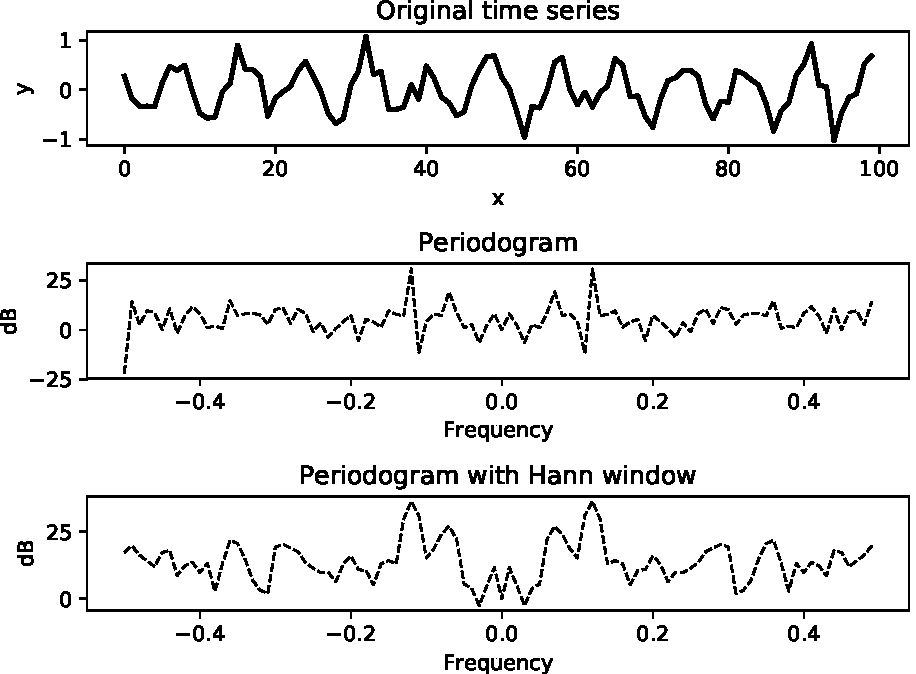
\includegraphics[width=0.70\textwidth]{taskb.pdf}
    \caption{Beregnet periodogram av tidsrekken.}
    \label{taskb}
\par}
\end{figure}


Her ser man at hann vinduet gir en glattere kurve, og lar ikke frekvense lekker over like mye som i det vanlige periodogrammet. Frekvensene ser ut til � v�re rundt 0.12 og 0.07.


\subsection{c}

Som nevnt i oppgave b s� fjerner vinduet mer av lekasjen i frekvensspekteret, fordi den har mindre sidelober enn den idelle w[k] = 1, men dette vil �ke bredden p� hovedloben slik at man f�r litt d�rligere oppl�sning. I figure(\ref{taskc}) har jeg ikke brukt dB skala slik at differansen er st�rre mellom styrken p� frekvensene. Her kan man tydelig se at vinduet hjelper med � se svakere periodisitetet i spectrumet. Periodogram ble laget ved bruk av Fourier transform som vist i ligning(\ref{Periodogram}).

\begin{equation}
    S(f) = \frac{1}{N}|\mathcal{F}\{x[n]\}|^{2}
    \label{Periodogram}
\end{equation}
der $\mathcal{F}$ er DTFT, \emph{Discrete Time Fourier Transform} og N er antall datapunkter. Ved bruk av vindu har vi ligning(\ref{wPeriodogram}).

\begin{equation}
    S_{w}(f) = \frac{1}{NU}|\mathcal{F}\{w[n]x[n]\}|^{2}
    \label{wPeriodogram}
\end{equation}

Her er $w[n]$ vinduet, i dette tilfelle er dette \emph{Hann window}. Vi bruker vindu for � minske spektral lekasje som kommer av at vi ikke kan ha en \emph{ekte} fourier transform som krever at signal vi har er uendelig langt. Derfor vil vi alltid ha en ende p� signal som man antar er null. Dette betyr at vi bruker et ideelt vindu med lengde M(signal lengden) n�r vi tar Fourier transform. N�r man ganger inn tids domenet s� konvolverer man i frekvensdomenet, og siden det ideele vinduet har store sidelober medf�rer dette til at man f�r ut n�rliggende frekvenser i hverandre og dermed gir spektral lekasje. Ved bruk av vindu som Hann vindu s� kan man redusere dette siden de har smalere sidelober.



\begin{figure}[hbt!]
    {\centering
        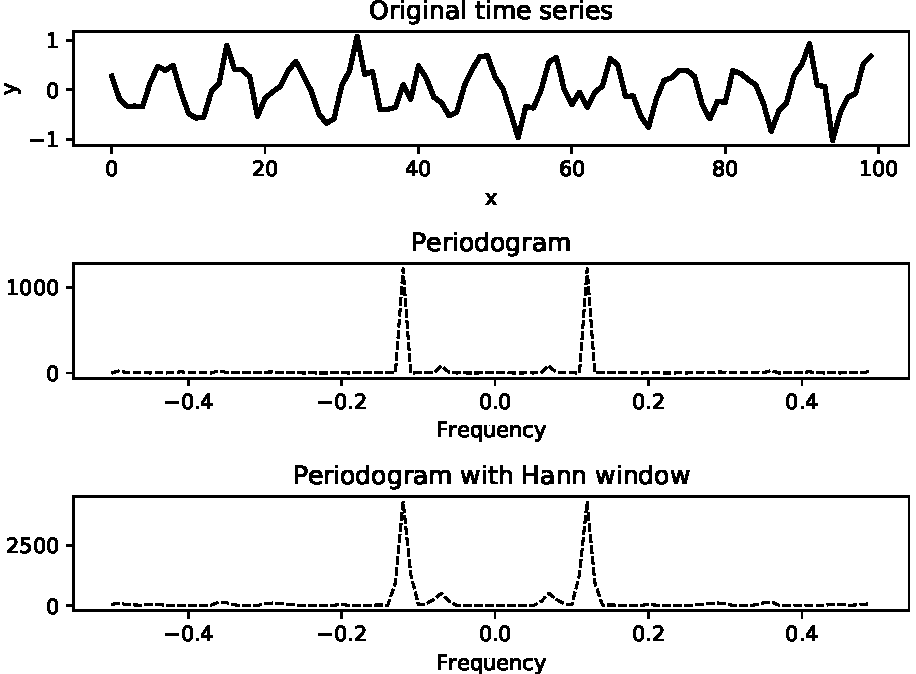
\includegraphics[width=0.70\textwidth]{taskc.pdf}
        \caption{Beregnet periodogram av tidsrekken uten dB skala.}
        \label{taskc}
    \par}
    \end{figure}

\subsection{d}

Ved � implementere WOSA (Weighted/Welchs overlapped segment averaging) p� tidsrekken fikk vi resultatet vist i figur(\ref{taskd}).

\begin{figure}[hbt!]
    {\centering
        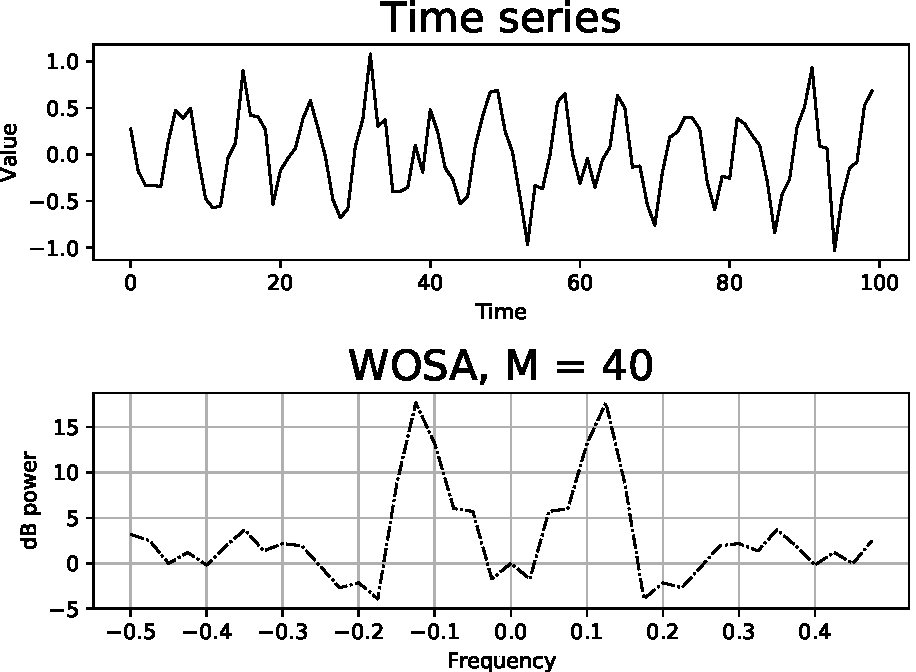
\includegraphics[width=0.70\textwidth]{taskd.pdf}
        \caption{WOSA med 50\% overlapp, N = 40}
        \label{taskd}
    \par}
    \end{figure}

Her ble hvert segment vektet som gir et kraftigere utslag der det er sterke periodisiteter i forhold til resten av spekteret. Her ser man at frekvensen p� ca $f \approx 0.15$ er sv�rt kraftig og $\approx 0.05$ viser seg ogs� \,ganske kraftig i forhold til alle de andre. Man kan se at frekvensene er mye tydligere i WOSA enn i periodogrammet og hann vinduet i dB skala som vist i figur(\ref{taskb}). 


\clearpage
\newpage
\section{2}

\subsection{a-b}

Her plottet vi sol-dataen som vist i �verste vindu i figur(\ref{task2}).


\begin{figure}[hbt!]
    {\centering
        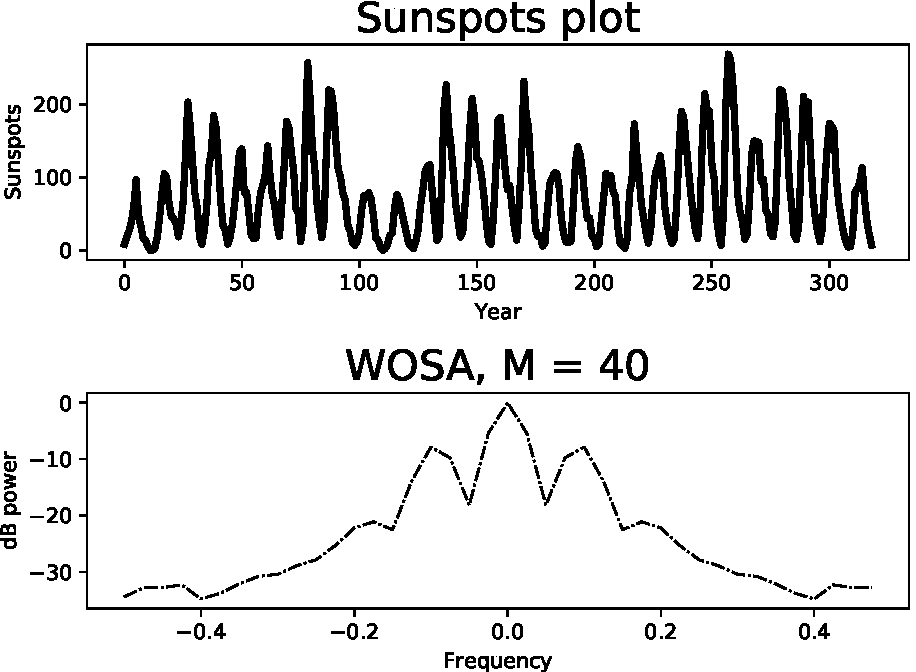
\includegraphics[width=0.70\textwidth]{task2.pdf}
        \caption{Soldata, WOSA med 50\% overlapp, N = 40}
        \label{task2}
    \par}
    \end{figure}

Her ble det brukt WOSA med 50\% overlapp og vindu-st�rrelse $N = 40$. Her ser man sterk DC og en frekvens p� rundt 0.1, $f \approx 0.1$. Dette gir en periode p� $T \approx 10$, noe som ser ut til � stemme hvis man teller antall topper som er $\approx 9$ per 100.


% --------------------------------------------------------------
%     Reference og appendix
% --------------------------------------------------------------
\section{Appendix}

\begin{figure}[H]
    \begin{lstlisting}
        import numpy as np 
        import matplotlib.pyplot as plt
        
        
        data = np.genfromtxt('tidsrekke_oblig2_oppg1.txt')
        
        
        def periodogram(x, dt):
            """Regular periodogram"""
            N = len(x)
            spectrum = np.abs(np.fft.fftshift(np.fft.fft(x))**2)
            spectrum *= dt/ N
            freq = np.fft.fftshift(np.fft.fftfreq(N, dt))
        
            return freq, spectrum
        
        
        def w_periodogram(x, dt):
            """Windowed periodogram"""
            N = len(x)
            n = np.arange(0,N,1)
            # Hann window
            window = (1/2)*(1 - np.cos(2*np.pi*n/(N-1)))
            U = (1/N)*np.sum(window**2)
            spectrum = np.abs(np.fft.fftshift(np.fft.fft(window*x)))**2
            spectrum *= (dt/(N*U))
            freq = np.fft.fftshift(np.fft.fftfreq(N, dt))
            return freq, spectrum
        
        dt = 1
        freq, spectrum = periodogram(data, dt)
        freqw, wspectrum = w_periodogram(data, dt)
        
        # Find index corresponding to f = 0 
        idx = np.where(freq == 0)
        widx = np.where(freqw == 0)
        
        # Plot
        fig, ax = plt.subplots(3,1)
        ax[0].plot(data, color = 'black', linewidth = 1)
        ax[0].set_title('Original time series')
        ax[0].set_xlabel('x')
        ax[0].set_ylabel('y')
        ax[1].plot(freq, 10*np.log10(spectrum/spectrum[idx]),'--', color = 'black', linewidth = 1)
        ax[1].set_title('Periodogram')
        ax[1].set_xlabel('Frequency')
        ax[1].set_ylabel('dB')
        ax[2].plot(freqw, 10*np.log10(wspectrum/wspectrum[widx]),'--', color = 'black', linewidth = 1)
        ax[2].set_title('Periodogram with Hann window')
        ax[2].set_xlabel('Frequency')
        ax[2].set_ylabel('dB')
        ax[1].set_xticks([x for x in np.arange(-0.5,0.5,0.1)])
        ax[2].set_xticks([x for x in np.arange(-0.5,0.5,0.1)])
        ax[1].grid()
        ax[2].grid()
        plt.tight_layout()
        plt.savefig('rapport/taskb.pdf', bbox_inches = 'tight',
            pad_inches = 0)
        plt.show()
        
    \end{lstlisting}
\caption{Task 1B-C}
\label{Task1B-Ccode}
\end{figure}


\begin{figure}[H]
    \begin{lstlisting}
        import matplotlib.pyplot as plt 
        import numpy as np 
        
        # Load file
        data = np.genfromtxt('tidsrekke_oblig2_oppg1.txt')
        
        
        def WOSA(x, M, dt = 1):
            """Implementation of WOSA"""
            n = np.arange(0, M, 1)
            window = (1/2)*(1 - np.cos(2*np.pi*n/(M-1)))
            U = (1/M)*np.sum(window**2)
            spectrum = np.zeros(M)
            n_windows = 2*int(len(x)/(M-1))
            for i in range(n_windows):
        
                # Start with window 0-40
                if i == 0:
                    spectrum_temp = np.fft.fftshift(np.fft.fft(window*x[0:40]))
                    plt.plot(x[0:40])
                    t = np.arange(0, 40, 1)
                    plt.plot(t, window)
        
        
                # Start overlapping
                else:
                    spectrum_temp = np.fft.fftshift(np.fft.fft(window*x[(i*int(M/2)):(i+2)*int(M/2)]))
                    plt.plot(x[0:(i+2)*int(M/2)])
                    t = np.arange((i*int(M/2)), (i+2)*int(M/2), 1)
                    plt.plot(t, window)
                spectrum += (dt/(M*U))*np.abs(spectrum_temp)**2        
            spectrum /= n_windows
            plt.show()
            freq = np.fft.fftshift(np.fft.fftfreq(M, dt))
            print('Number of windows: %s'%n_windows)
            return freq, spectrum
        
        M = 40
        dt = 1
        freq, spectrum = WOSA(data, M)
        # Find index corresponding to f = 0 
        idx = np.where(freq == 0)
        
        # Plot
        fig, ax = plt.subplots(2,1)
        ax[0].plot(data, linewidth = '1', color = 'black')
        ax[0].set_title('Time series', fontsize = '20')
        ax[0].set_ylabel('Value')
        ax[0].set_xlabel('Time')
        ax[1].plot(freq, 10*np.log10(spectrum/spectrum[idx]), '-.', linewidth = '1', color = 'black')
        ax[1].set_title('WOSA, M = %s'%M, fontsize = '20')
        ax[1].set_xlabel('Frequency')
        ax[1].set_ylabel('dB power')
        ax[1].set_xticks([x for x in np.arange(-0.5,0.5,0.1)])
        ax[1].grid()
        plt.tight_layout()
        plt.savefig('rapport/taskd.pdf', bbox_inches = 'tight',
            pad_inches = 0)
        plt.show() 
    \end{lstlisting}
\caption{Task D}
\label{TaskDcode}
\end{figure}



\begin{figure}[H]
    \begin{lstlisting}
        import os
        import pandas as pd
        import numpy as np 
        import matplotlib.pyplot as plt
        
        filedir = os.path.dirname(__file__)
        filename = 'SN_y_tot_V2.0.txt'
        
        file = os.path.join(filedir, filename)
        
        # load file
        datatable = pd.read_csv(file,sep='\t',header=None,engine='python')
        time = np.zeros(len(datatable))
        sunspots = np.zeros(len(datatable))
        
        for i in range(len(datatable)):
             time[i] = datatable.values[i,0][0:6]
             sunspots[i] = datatable.values[i,0][8:13]
        
        
        def WOSA(x, M, dt = 1):
            """Implementation of WOSA"""
            n = np.arange(0, M, 1)
            window = (1/2)*(1 - np.cos(2*np.pi*n/(M-1)))
            U = (1/M)*np.sum(window**2)
            spectrum = np.zeros(M)
            n_windows = 2*int(len(x)/(M-1))-1
            x = np.pad(x, (0, M), 'constant')
            for i in range(n_windows):
                # Start with window 0-40
                if i == 0:
                    spectrum_temp = np.fft.fftshift(np.fft.fft(window*x[0:40]))
                    plt.plot(x[0:40])
                    t = np.arange(0, 40, 1)
                    plt.plot(t, 200*window)
                
                # Start overlapping
                else:
                    spectrum_temp = np.fft.fftshift(np.fft.fft(window*x[(i*int(M/2)):(i+2)*int(M/2)]))
                    plt.plot(x[0:(i+2)*int(M/2)])
                    t = np.arange((i*int(M/2)), (i+2)*int(M/2), 1)
                    plt.plot(t, 200*window)
                spectrum += (dt/(M*U))*np.abs(spectrum_temp)**2   
            spectrum /= n_windows
            plt.show()
            plt.close()
            freq = np.fft.fftshift(np.fft.fftfreq(M, dt))
            print('Number of windows: %s'%n_windows)
            return freq, spectrum
        
        M = 40
        dt = 1
        freq, spectrum = WOSA(sunspots, M)
        # Find index corresponding to f = 0 
        idx = np.where(freq == 0)
        
        # plot
        fig, ax = plt.subplots(2,1)
        ax[0].plot(sunspots, linewidth = '3', color = 'black')
        ax[0].set_title('Sunspots plot', fontsize = '20')
        ax[0].set_ylabel('Sunspots')
        ax[0].set_xlabel('Year')
        ax[1].plot(freq, 10*np.log10(spectrum/spectrum[idx]), '-.', linewidth = '1', color = 'black')
        ax[1].set_title('WOSA, M = %s'%M, fontsize = '20')
        ax[1].set_xlabel('Frequency')
        ax[1].set_ylabel('dB power')
        ax[1].set_xticks([x for x in np.arange(-0.5,0.5,0.1)])
        ax[1].grid()
        plt.tight_layout()
        plt.savefig('rapport/task2.pdf', bbox_inches = 'tight',
            pad_inches = 0)
        plt.show() 
    \end{lstlisting}
\caption{Task 2 code}
\label{Task2code}
\end{figure}



\section{Referanser}
\begingroup
\renewcommand{\section}[2]{}%
%\renewcommand{\chapter}[2]{}% for other classes
\bibliographystyle{plainnat}
\bibliography{bibl}
\endgroup



% --------------------------------------------------------------
%     You don't have to mess with anything below this line.
% --------------------------------------------------------------
 





\end{document}


